% This is the Duke University Statistical Science LaTeX thesis template.
% It has been adapted from the Reed College LaTeX thesis template. The
% adaptation was done by Mine Cetinkaya-Rundel (MCR). Some of the comments
% that are specific to Reed College have been removed.
%
% Most of the work on the original Reed College document class and template
% was done by Sam Noble (SN). Later comments etc. by Ben Salzberg (BTS).
% Additional restructuring and APA support by Jess Youngberg (JY).
%
% See https://www.reed.edu/cis/help/latex/ for help. There are a
% great bunch of help pages there, with notes on
% getting started, bibtex, etc. Go there and read it if you're not
% already familiar with LaTeX.
%
% Any line that starts with a percent symbol is a comment.
% They won't show up in the document, and are useful for notes
% to yourself and explaining commands.
% Commenting also removes a line from the document;
% very handy for troubleshooting problems. -BTS

%%
%% Preamble
%%
% \documentclass{<something>} must begin each LaTeX document
\documentclass[12pt,twoside]{dukestatscithesis}
% Packages are extensions to the basic LaTeX functions. Whatever you
% want to typeset, there is probably a package out there for it.
% Chemistry (chemtex), screenplays, you name it.
% Check out CTAN to see: http://www.ctan.org/
%%
\usepackage{graphicx,latexsym}
\usepackage{amsmath}
\usepackage{amssymb,amsthm}
\usepackage{longtable,booktabs,setspace}
\usepackage{chemarr} %% Useful for one reaction arrow, useless if you're not a chem major
\usepackage[hyphens]{url}
% Added by CII
\usepackage{hyperref}
\usepackage{lmodern}
\usepackage{float}
\floatplacement{figure}{H}
% End of CII addition
\usepackage{rotating}

% Next line commented out by CII
%%% \usepackage{natbib}
% Comment out the natbib line above and uncomment the following two lines to use the new
% biblatex-chicago style, for Chicago A. Also make some changes at the end where the
% bibliography is included.
%\usepackage{biblatex-chicago}
%\bibliography{thesis}


% Added by CII (Thanks, Hadley!)
% Use ref for internal links
\renewcommand{\hyperref}[2][???]{\autoref{#1}}
\def\chapterautorefname{Chapter}
\def\sectionautorefname{Section}
\def\subsectionautorefname{Subsection}
% End of CII addition

% Added by CII
\usepackage{caption}
\captionsetup{width=5in}
% End of CII addition

% \usepackage{times} % other fonts are available like times, bookman, charter, palatino


% To pass between YAML and LaTeX the dollar signs are added by CII
\title{Exploring Geometric Anisotropy for Point-Referenced Spatial Data}
\author{Angie Shen}
% The month and year that you submit your FINAL draft TO THE LIBRARY (May or December)
\date{December 2017}
\advisor{Dr.~Alan Gelfand}
\institution{Duke University}
\degree{Bachelor of Science in Statistical Science}
\committeememberone{Dr.~Colin Rundel}
\committeemembertwo{Dr.~Katherine Heller}
\dus{Dr.~Mine Çetinkaya-Rundel}
%If you have two advisors for some reason, you can use the following
% Uncommented out by CII
% End of CII addition

%%% Remember to use the correct department!
\department{Department of Statistical Science}

% Added by CII
%%% Copied from knitr
%% maxwidth is the original width if it's less than linewidth
%% otherwise use linewidth (to make sure the graphics do not exceed the margin)
\makeatletter
\def\maxwidth{ %
  \ifdim\Gin@nat@width>\linewidth
    \linewidth
  \else
    \Gin@nat@width
  \fi
}
\makeatother

\renewcommand{\contentsname}{Table of Contents}
% End of CII addition

\setlength{\parskip}{0pt}

% Added by CII

\providecommand{\tightlist}{%
  \setlength{\itemsep}{0pt}\setlength{\parskip}{0pt}}

\Acknowledgements{

}

\Dedication{

}

\Preface{

}

\Abstract{
Isotropic covariance functions are routinely adopted in specifying
models for point-referenced spatial data. Implicit in such modeling is
the assumption that spatial dependence is not directional. Geometric
anisotropic models offer a class of specifications which incorporate
directional dependence. They have received sparse attention in the
literature because their associated number of parameters increase and
become difficult to identify as we increase richness of the function.
Adopting a Bayesian framework, this paper attempts to illuminate when
and how much such models for random effects in geostatistical settings
improve predictive performance. We show that geometric anisotropy yields
better predictive performance when the data significantly departs from
isotropy (anisotropy ratio is much greater than one), and that the
improvement is more prominent when spatial variance is greater than pure
error. The improvement in predictive performance is illustrated through
simulation investigation as well as modeling data on scallop catches. We
implement full Bayesian inference for model parameters using Markov
chain Monte Carlo with a Metropolis-Hastings algorithm, adding kriging
using composition sampling.
}

	\usepackage{tikz}
	\usepackage{amsmath}
	\usepackage{amsfonts}
	\usepackage{graphicx}
	\usepackage{caption}
	\usepackage{subcaption}
	\usepackage{float}
	\usepackage{palatino}
	\usepackage{times}
	\usepackage{color}
	\usepackage[utf8]{inputenc}
	\usepackage[english]{babel}
	\usepackage[round]{natbib}
	\usepackage{pbox}
	\usepackage{tabularx}
	\bibliographystyle{chicago}
% End of CII addition
%%
%% End Preamble
%%
%

\usepackage{amsthm}
\newtheorem{theorem}{Theorem}[chapter]
\newtheorem{lemma}{Lemma}[chapter]
\theoremstyle{definition}
\newtheorem{definition}{Definition}[chapter]
\newtheorem{corollary}{Corollary}[chapter]
\newtheorem{proposition}{Proposition}[chapter]
\theoremstyle{definition}
\newtheorem{example}{Example}[chapter]
\theoremstyle{definition}
\newtheorem{exercise}{Exercise}[chapter]
\theoremstyle{remark}
\newtheorem*{remark}{Remark}
\newtheorem*{solution}{Solution}
\begin{document}

% Everything below added by CII
  \maketitle

\frontmatter % this stuff will be roman-numbered
\pagestyle{empty} % this removes page numbers from the frontmatter



  \hypersetup{linkcolor=black}
  \setcounter{tocdepth}{2}
  \tableofcontents

  \listoftables

  \listoffigures
  \begin{abstract}
    Isotropic covariance functions are routinely adopted in specifying
    models for point-referenced spatial data. Implicit in such modeling is
    the assumption that spatial dependence is not directional. Geometric
    anisotropic models offer a class of specifications which incorporate
    directional dependence. They have received sparse attention in the
    literature because their associated number of parameters increase and
    become difficult to identify as we increase richness of the function.
    Adopting a Bayesian framework, this paper attempts to illuminate when
    and how much such models for random effects in geostatistical settings
    improve predictive performance. We show that geometric anisotropy yields
    better predictive performance when the data significantly departs from
    isotropy (anisotropy ratio is much greater than one), and that the
    improvement is more prominent when spatial variance is greater than pure
    error. The improvement in predictive performance is illustrated through
    simulation investigation as well as modeling data on scallop catches. We
    implement full Bayesian inference for model parameters using Markov
    chain Monte Carlo with a Metropolis-Hastings algorithm, adding kriging
    using composition sampling.
  \end{abstract}

\mainmatter % here the regular arabic numbering starts
\pagestyle{fancyplain} % turns page numbering back on

\chapter*{Introduction}\label{introduction}
\addcontentsline{toc}{chapter}{Introduction}

Researchers in diverse areas such as climatology, ecology and
environmental health are increasingly interested in analyzing data that
are geographically referenced. For example, epidemiologists may be
interested in studying the number of lung cancer incidents by county and
state. Ecologists may be interested in the location of a particular
species of trees in a forest. Researchers are often interested in
statistical inference tasks, such as modeling of trends and correlation
structures, estimation of underlying model parameters, hypothesis
testing, model comparison and selection, and prediction of observations
at unobserved locations (kriging).

With the advancement of Markov chain Monte Carlo (MCMC) computing,
Bayesian modeling approaches have become increasingly common, as they
enable hierarchical model structures where prior belief is updated with
new information, as well as natural quantification of uncertainty
through sampling schemes. The (Banerjee, Carlin, \& Gelfand, 2014) text
presents a thorough treatment of hierarchical Bayesian approaches for a
variety of complex spatial data problems.

One common type of spatial data is \(\textit{point-referenced}\) data,
often referred to as \(\textit{geostatistical}\) data, where we observe
realizations of a spatial stochastic process at a fixed set of
locations. We are often interested in a geographical distribution for
the realizations that accounts for spatial correlation, typically in the
presence of spatially referenced covariates. The simplest choices for
modeling spatial correlation are \(\textit{isotropic}\) covariance
functions, where we assume spatial correlation between locations depends
only on the distance between locations. In cases where this assumption
does not hold, i.e., spatial correlation varies by direction, we can
consider \(\textit{anisotropic}\) covariance functions which depend on
the separation vector between locations.

In the literature we find several notions of anisotropy, e.g., sill,
nugget, and geometric anisotropy (Zimmerman, 1993). From a generative
modeling perspective, the most useful form of anisotropy is
\(\textit{Geometric Anisotropy}\), where coordinates are linearly
transformed, i.e., rotated and stretched, to allow for different
magnitudes of correlation in different directions. (Budrikaite \&
Ducinskas, 2005) explored different forms of geometric anisotropic
variograms. (Eriksson \& Siska, 2000) provided the geometrical details
for modeling various types of anisotropy (range, sill, power, slope,
nugget) on an ellipse. (Allard, Senoussi, \& Porcu, 2016) derived a
directional representation of anisotropies to build a large class of
models that include and go beyond classical anisotropies such as the
geometric and zonal ones. (Porcu, Gregori, \& Mateu, 2006) incorporated
anisotropy into spatio-temporal covariance models. (Ecker \& Gelfand,
1999) proposed a Bayesian methodology for simultaneously estimating the
linear transformation of the coordinates and other variogram parameters,
which also allows full inference for any characteristic of the
geometrically anisotropic model. Following (Ecker \& Gelfand, 1999) who
proposed to use objective, independent priors for model parameters,
(Kazianka, 2013) developed default priors and studied their posterior
propriety.

This paper attempts to illuminate when and how much geometric
anisotropic (henceforth anisotropic) models for random effects in
geostatistical settings improve predictive performance. We use a
transformation matrix parametrized by a decay parameter, a rotation
angle and an anisotropy ratio. In the form of a simulation study, we
compare the predictive performance of isotropic and anisotropic models
for data generated under anisotropy. We also test the sensitivity of the
models to different parameter values of the data generating model,
including different sample sizes, different choices of anisotropy ratio,
and different scales and ratios of spatial variance and pure error. We
find that geometric anisotropy yields better predictive performance when
the data significantly departs from isotropy (anisotropy ratio is much
greater than one), and the improvement is more prominent when spatial
variance is greater than pure error. We use Metropolis Hastings
algorithm to perform full Bayesian inference for all model parameters.
We then fit isotropic and anisotropic models to data on scallop catches
used in (Ecker \& Gelfand, 1999) which have been shown to suggest
anisotropic behavior. We show that the anisotropic model performs better
in terms of empirical coverage, predictive mean squared error and
continuous rank probability score.

The paper proceeds as follows. Section 2 formally defines the isotropic
and geometric anisotropic models we use for point-referenced data.
Section 3 details our model fitting algorithm and distribution theory
for making predictions. Section 4 lays out the metrics we use for model
comparison. Section 5 demonstrates the simulation exercise with
associated results. Section 6 presents modeling results for scallop
catches data. Finally, Section 7 discusses future work.

\chapter{Models}\label{models}

\section{Point-Level Models}\label{point-level-models}

Suppose \(\{Y(s): s \in D\}\) is a stochastic process where \(D\) is a
fixed subset of \(r\)-dimensional Euclidean space. When \(r=2\), we say
that \(Y(s)\) is a \(\textit{spatial process}\). Data generated by such
spatial process \(Y(s)\) where \(s\) varies continuously over \(D\) is
\(\textit{point-referenced}\) data. For example, \(Y(s)\) may represent
pollutant level over a region, and we observe pollutant measurements at
a finite set of locations\(\{s_1, ..., s_n\}\) where there are
monitoring stations. Even though \(Y(s)\) exists on an infinite
dimensional function space, in reality we can only observe data at a
finite number of locations. The data is a partial realization of the
spatial process. The problem facing statisticians is to make inference
about the spatial process \(Y(s)\) and prediction at new locations based
on this partial realization.

We model \(Y(s)\) with a \(\textit{Gaussian Process}\). Suppose our
spatial process has a mean \(\mu(s) = E(Y(s))\) associated with it and
the variance of \(Y(s)\) exists for all \(s \in D\). \(Y(s)\) is said to
be \(\textit{Gaussian}\) if for any \(n \ge 1\) and any set of \(n\)
sites \(\{s_1, ..., s_n\}\), \(Y = (Y(s_1), ..., Y(s_n))^T\) has a
multivariate normal distribution. The remarkable feature of Gaussian
Process models is that, despite only observing the spatial surface at a
finite number of locations, we can infer about the process at an
uncountable number of locations by specifying the association between
pairs of locations through \(\textit{structured}\) dependence. Suppose
we assume the random variables at two locations depend on the
\(\textit{distance}\) of the locations. If we assume spatial correlation
is a function solely of the distance \(d_{ii'}\) between \(s_i\) and
\(s_{i'}\), the covariance function is \(\textit{isotropic}\). One
commonly used isotropic covariance specification is the exponential
model, where the covariance between measurements at two locations is an
exponential function decreasing in the distance between the two
locations.

Suppose we have observations
\(\textbf{Y} = \{Y(s_1), . . . , Y(s_n)\}\). We assume a multivariate
normal model where
\begin{equation}
\textbf{Y} \sim N_n(\mu \textbf{1},  \Sigma(\theta))
\end{equation}
where \(N_n\) denotes the n-dimensional normal distribution, \(\mu\) is
the global mean\footnote{We assume a constant mean surface here and in
  the sequel since our focus is on the effects of the choice of
  covariance function.}, and \((\Sigma(\theta))_{ii'}\) gives the
covariance between \(Y(s_i)\) and \(Y(s_{i'})\).

If we use an exponential correlation function,
\begin{equation}
\Sigma{(\theta)}_{ii'} = \begin{cases}
\sigma^2 + \tau^2 & \text{if $d_{ii'}=0$}\\
\sigma^2\text{exp}(-\phi d_{ii'}) & \text{if $d_{ii'}>0$}
\end{cases}
\end{equation}
where \(d_{ii'}\) is the distance between site \(s_i\) and \(s_{i'}\),
\(\phi > 0\) is the \(\textit{decay parameter}\) (1/\(\phi\) is the
\(\textit{range}\) parameter), \(\sigma^2 > 0\) is
\(\textit{partial sill}\) or spatial variance, \(\tau^2 > 0\) is
\(\textit{nugget}\) or pure error, and \(\tau^2 + \sigma^2\) is
\textit{sill}. The parameters of the covariance matrix are
\(\theta = (\sigma^2, \tau^2, \phi)^T\).

\section{Isotropy}\label{isotropy}

Suppose we observe \(\{Y(s): s \in D \subseteq \mathbb{R}^r\}\). For any
\(h \in \mathbb{R}^r\), \textit{intrinsic stationarity} assumes that
\(E(Y(s+h) - Y(s)) = 0\) and that Var(\(Y(s+h)-Y(s)\)) is a function of
the separation vector \(h\), denoted by \(2\gamma(h)\), the
\textit{variogram}. The stronger assumption of
\textit{weak stationarity} asserts that \(E(Y(s)) = \mu\) (the mean is
constant) and Cov\((Y(s), Y(s+h))=C(h)\), and implies
\textit{intrinsic stationarity} with \(\gamma(h)=C(0) - C(h)\). Under
\textit{isotropy}, the \textit{semivariogram} function \(\gamma(h)\)
depends on the separation vector only through its length
\(d=\lVert h \rVert\). That is, the variogram is a function of the
Euclidean distance \(d\) between two sites. The \textit{sill} is
\(\lim_{d\to\infty}2\gamma(d)\). The \textit{range} is the distance at
which the sill is reached; sites separated by distances larger than the
range are uncorrelated. The \textit{effective range} is defined as the
distance such that Corr\((Y(s_i), Y(s_j))=0.05\). The \textit{nugget} is
\(\lim_{d\to0}2\gamma(d)\), which need not be zero, to allow for
measurement error and microscale variability.

\section{Geometric Anisotropy}\label{geometric-anisotropy}

Isotropic variograms are popular because of their simplicity and
interpretability. However, in many cases correlation function does not
simply depend on the distance between locations, but depends on
separation vector between locations. As a result, association depends
upon direction. Here we explore covariance functions that are stationary
but not isotropic. When the variogram is a function of both length and
orientation of the separation vector \(h\), the process \(Y(s)\) is said
to be \(\textit{anisotropic}\). That is, the semivariogram is
\(\gamma(h)\) rather than \(\gamma(\lVert h \rVert)\).

Following (Zimmerman, 1993), anisotropy can take three general forms:
\textit{sill anisotropy}, \textit{nugget anisotropy}, and
\textit{range anisotropy}. When
\(\lim_{a\to\infty}\gamma(ah/\rVert h \rVert)\) depends on the
separation vector \(h\), the situation is referred to as sill
anisotropy. When \(\lim_{a\to0}\gamma(ah/\rVert h \rVert)\) depends on
\(h\), the situation is referred to as nugget anisotropy. Nugget
anisotropy is typically ascribed to correlated measurement errors. A
third type of anisotropy is range anisotropy where the range depends
upon direction. This is the form most often seen in practice. A common
case of range anisotropy is geometric anisotropy where we set
\begin{equation}
Cov(s - s') = \sigma^2\rho((s - s')^TB(s - s'))\\
\end{equation}
where \(B\) is a positive semidefinite matrix and \(\rho\) is a valid
correlation function in \(R^r\). When \(r=2\), \(B\) is \(2 \times 2\),
and the correlation specification will have three parameters rather than
one decay parameter. \(B = \phi I\) corresponds to isotropy and arises
from a linear transformation of coordinates under a general \(B\). The
contour corresponding to \(\rho = 0.05\) provides the range in each
spatial direction, and its shape is described by an ellipse.

As detailed in (Eriksson \& Siska, 2000), for sites \(s_i\) and \(s_j\),
we define the covariance function as:
\begin{equation}
\Sigma{(\theta)}_{ij} = \sigma^2\text{exp}(-\phi (h_{ij}^{T}Bh_{ij})^{1/2}) + \tau^2 I(i = j)\\
\end{equation}
where
\begin{equation}
B = AA^{T}, A =
 \begin{bmatrix}
\text{cos}(\alpha) & \text{sin}(\alpha) \\
-\text{sin}(\alpha) & \text{cos}(\alpha)
\end{bmatrix}
\begin{bmatrix}
1/r & 0\\
0 & 1
\end{bmatrix}
\end{equation}
\textbackslash{} where \(h_{ij} = s_i - s_j\). Here, \(\alpha\) is
orientation of the associated ellipse and \(r\) is anisotropy ratio
(ratio of the major axis to the minor axis of the ellipse). The \(B\)
matrix rotates and stretches the range of the covariance. Again, when
\(B\) is a constant times the identity matrix, the covariance function
is isotropic.

The range \(c\) in direction \(\theta\) is obtained by taking a unit
vector in direction \(\theta\), \(h_{\theta}\), and then solving
\(\rho(c_\theta^2 h_{\theta}^{T}Bh_{\theta})=.05\) for \(c_\theta\). In
the case of the exponential correlation function, we have
\begin{equation}
\text{exp}(-c_\theta (h_\theta^{T}Bh_\theta)^{1/2}) = 0.05 \\
\end{equation}
where \(h_\theta = (cos(\theta), sin(\theta))\).

Figure \ref{fig:rangessim} shows spatial ranges in every direction from
\(0^\circ\) to \(360^\circ\) with different combinations of the rotation
angle and anisotropy ratio. The right panel shows the range in polar
coordinates, forming ellipses. We can see that when the anisotropy axis
ratio is closer to 1, the range does not vary much by direction and
associated ellipse is closer to a circle.
\begin{figure}
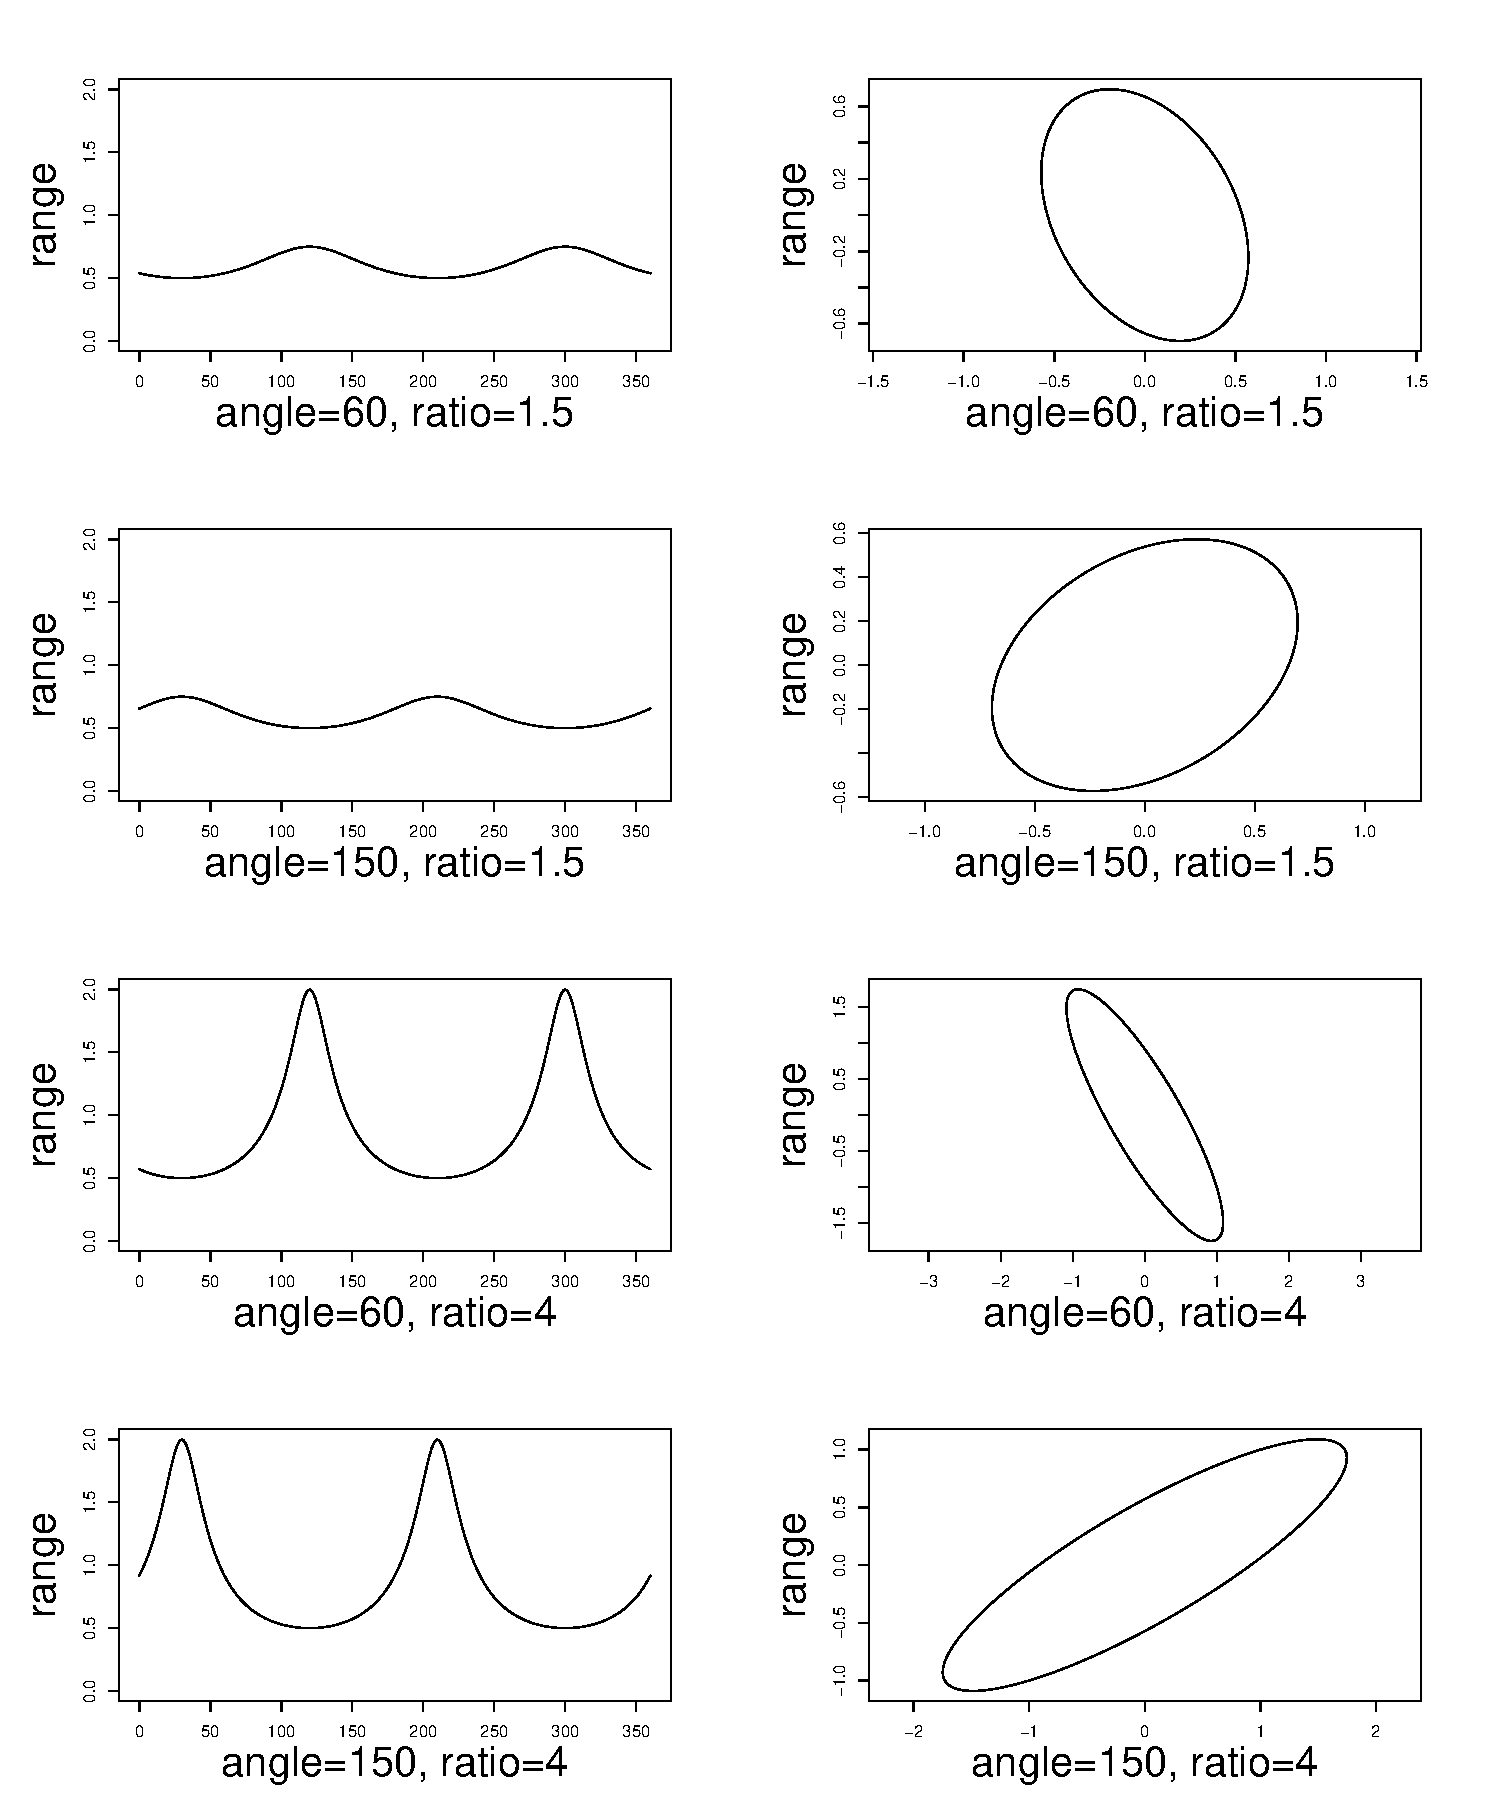
\includegraphics[scale=0.6]{figure/ranges_sim} \caption{Spatial range with different specifications of rotation angle and anisotropy ratio}\label{fig:rangessim}
\end{figure}
\chapter{Methodology}\label{methodology}

\section{Model Fitting}\label{model-fitting}

We use the Bayesian framework to perform inference on model parameters
and predictions for new locations. Not only do we simultaneously
estimate for the ratio of major axis to minor axis of the ellipse, the
angle of orientation of the ellipse with respect to the x-axis, the
decay parameter, and the additional variogram parameters, but we provide
complete inference in the form of a posterior distribution for each
parameter. In addition, the Bayesian framework enables incorporation of
prior information. If a priori, the process is expected to exhibit
geometric anisotropy whose characteristics we can quantify, this
information is easily built into the prior specifications and the model.

We model the data with a Gaussian Process
\begin{equation}
\textbf{Y} \sim N_n(\mu \textbf{1},  \Sigma(\theta))
\end{equation}
where \(\Sigma(\theta)\) is specified by (4) and (5), and
\(\theta = (\sigma^2, \tau^2, \phi, \alpha, r)^T\). Under the likelihood
implied by (7) for a set of say \(n\) locations, we complete the
Bayesian formulation by assuming the prior takes the form
\begin{equation}
\pi(\mu, \theta) = \pi(\mu, \sigma^2, \tau^2, \phi, \alpha, r) = \pi(\mu)\pi(\sigma^2)\pi(\tau^2)\pi(\phi)\pi(\alpha)\pi(r),
\end{equation}
i.e., assuming all the parameters are independent.

We use a weak \(N(0, 1000)\) prior for \(\mu\). We use vague inverse
gamma distributions for the variances \(\sigma^2\) and \(\tau^2\) and
anisotropy ratio \(r\) with shape and scale parameters both equal to
one, implying no prior mean or variance. We put a uniform\((0, \pi)\)
prior on rotation angle \(\alpha\) and a uniform\((0.1D, 0.5D)\) on
range \(1/\phi\), where \(D\) is the maximum distance between locations.

We use a Metropolis-Hastings sampling algorithm to obtain samples from
the posterior distribution of all parameters \(p(\theta|y)\). The
Metropolis-Hastings algorithm is a Markov chain Monte Carlo (MCMC)
method for obtaining a sequence of random samples from a probability
distribution for which direct sampling is difficult. As more and more
sample values are produced, the distribution of values more closely
approximates the desired posterior distribution \(p(\theta|y)\).

Intuitively, assume we have a collection of
\(\{\theta^{(1)}, . . . , \theta^{(s)}\}\). To generate a new value
\(\theta^{(s+1)}\), we sample a new value \(\theta^*\) that is nearby
\(\theta^{(s)}\) and consider whether to accept the sampled \(\theta^*\)
into the collection of \(\theta's\). We sample \(\theta^*\) from a
proposal distribution \(J\) centered on \(\theta^{(s)}\), and accept
\(\theta^*\) if \(p(\theta^*|y) > p(\theta^{(s)}|y)\). If
\(p(\theta^*|y) < p(\theta^{(s)}|y)\), we accept \(\theta^*\) with some
probability. In Metropolis algorithm, the proposal distribution \(J\) is
symmetric. That is,
\(J(\theta^*|\theta^{(s)})=J(\theta^{(s)}|\theta^*)\). In
Metropolis-Hastings, J may not be symmetric.

The Metropolis-Hastings algorithm proceeds as follows.
\begin{enumerate}
\item Sample $\theta^* \sim J(\theta|\theta^{(s)})$
\item Compute acceptance ratio $r$:

$r = \displaystyle\frac{p(\theta^*|y)}{p(\theta^{(s)}|y)} \times \frac{J(\theta^*|\theta^{(s)})}{J(\theta^{(s)}|\theta^*)} = \displaystyle\frac{p(y|\theta^*)p(\theta^*)}{p(y|\theta^{(s)})p(\theta^{(s)})}\times \frac{J(\theta^*|\theta^{(s)})}{J(\theta^{(s)}|\theta^*)}$

(In the case of Metropolis, $\displaystyle\frac{J(\theta^*|\theta^{(s)})}{J(\theta^{(s)}|\theta^*)}=1$)
\item Sample $u \sim \text{Uniform}(0, 1)$. Set $\theta^{(s+1)} = \theta^*$ if $u < r$ and set $\theta^{(s+1)} = \theta^s$ otherwise.
\end{enumerate}
We use appropriate proposal distributions for different parameters. For
rotation angle \(\alpha\), we generate normal proposals mod \(\pi\). For
anisotropy ratio \(r\), we generate proposals from truncated normal
distribution from \(0\) to \(\infty\) as \(r\) can only be positive. We
also experimented with using log normal proposal for \(r\), but the
sampler behaved poorly as it frequently generated extremely big values.
For \(\sigma^2\), \(\tau^2\) and \(\phi\) we generate proposals from log
normal distribution. Finally, we generate \(\mu\) from a normal
distribution. Table 1 lists the proposal and prior distributions we use
for all the parameters.

Because \(\alpha\) and \(r\) are highly correlated, we update them
jointly. We tune the variances of the proposal distributions so that we
accept around \(25\%\) of all generated samples to achieve optimal
efficiency of the sampler. If proposals vary too much, the sampler will
reject too many samples which is inefficient. If proposals vary too
little, the chain of samples will not move very much and might get stuck
in a local mode.
\begin{table}[H]
\centering
\setlength{\extrarowheight}{10pt}
\begin{tabular}{|c|c|c|}
\hline
 & Proposal Distribution & Prior Distribution\\[8pt]
\hline
$\alpha$ & Normal (mod $\pi$) & Uniform$(0, \pi$)\\[8pt]
\hline
$r$ & Truncated Normal $_{(0, +\infty)}$& Inverse Gamma$(1,1)$\\[8pt]
\hline
$\sigma^2$ & Log Normal & Inverse Gamma$(1,1)$\\[8pt]
\hline
$\tau^2$ & Log Normal & Inverse Gamma$(1,1)$\\[8pt]
\hline
$\phi$ & Log Normal & Uniform $(3/0.5D, 3/0.2D)$\\[8pt]
\hline
$\mu$ & Normal & Normal$(0, 1000)$\\[8pt]
\hline
\end{tabular}
\caption{Proposal and prior distributions for Metropolis algorithm}
\end{table}
\section{Kriging}\label{kriging}

Spatial prediction in the point-referenced data setting is often
referred to as \textit{kriging}. Given observations
\(Y = (Y(s_1), ..., Y(s_n))\), how do we predict \(Y(s_0)\), where
\(s_0\) is a site that has not been observed? An observation at location
we want to predict \(s_0\) follows the following distribution:
\begin{eqnarray*}
y(s_o) = \mu + w(s_0) + \epsilon(s)
\end{eqnarray*}
There are two ways of formulating the posterior predictive distribution.
The first way samples spatial random effect w:
\begin{gather*}
[Y(s_0)|Y] = \int [Y(s_0)|w(s_0),\theta][w(s_0)|w, \theta][w|\theta, Y][Y|\theta]\\
[w|\theta, Y] = N((\frac{1}{\tau^2}I + \Sigma^{-1})^{-1}\frac{1}{\tau^2}(Y-\mu\textbf{1}), (\frac{1}{\tau^2}I + \Sigma^{-1})^{-1})\\
[w(s_0)|w] = N(r^{T}\Sigma^{-1}w, \sigma^{2}-r^{T}\Sigma^{-1}r)\\
[Y(s_0)|w(s_0),\theta] = N(\mu + w(s_0), \tau^2)
\end{gather*}
where \(r\) is the \(n \times 1\) covariance matrix between the new
location \(s_0\) and all other observed locations,
cov\((w(s_0), w(s_i)), i=1, 2, ...n\). \(\Sigma\) is the \(n \times n\)
covariance matrix between the random effects at the observed locations,
\((w(s_1),...w(s_n))\).\textbackslash{}\textbackslash{}

The second way marginalizes out spatial random effect w:
\begin{gather*}
[Y(s_0)|Y] = \int [Y(s_0)|Y,\theta][\theta|Y]\\
[Y(s_0)|Y,\theta][\theta|Y] = N(\mu + r^{T}(\Sigma + \tau^2I)^{-1}(Y-\mu\textbf{1}), \sigma^2+\tau^2-r^{T}(\Sigma+\tau^2I)^{-1}r)
\end{gather*}
We use the second approach in our algorithm as it has been shown to
yield better sampling behavior.

\chapter{Model Comparison}\label{model-comparison}

We use the following three metrics for model comparison.

\section{Predictive Mean Squared
Error}\label{predictive-mean-squared-error}

The predictive mean squared error measures the mean squared difference
between the predicted value and the observed value averaged over all
hold out locations.
\begin{eqnarray*}
PMSE=\frac{1}{n}\sum(\hat{Y} - Y_{obs})^2
\end{eqnarray*}
In the Bayesian context, \(\hat{Y}\) for each location is the posterior
predictive mean. We then average the squared difference between
\(\hat{Y}\) and the observed value over all hold out locations.

\section{Empirical Coverage}\label{empirical-coverage}

Empirical coverage assesses how well credible intervals, derived from
the posterior predictive distributions of the predictions, capture the
observed values of the hold out sample. Suppose we obtain 90\% credible
intervals from the posterior predictive distributions for each of the
hold out locations. If the credible intervals capture the observed value
for \$\textless{}\$90\% hold out locations, we have
\textit{under coverage}. If the credible intervals capture the observed
value for \$\textgreater{}\$90\% hold out locations, we have
\textit{over coverage}. Since the empirical coverage is random, we will
criticize the adequacy of the model when the departure from the nominal
coverage is consequential.

\section{Continuous Rank Probability Score
(CRPS)}\label{continuous-rank-probability-score-crps}

To examine how concentrated the predictive distribution of \(Y(s_0)\) is
around the observed value, we use the Continuous Rank Probability Score
(CRPS) metric, the squared integrated distance between the predictive
distribution and the degenerate distribution at the observed value,
\begin{equation*}
CRPS(F,y) = \int_{-\infty}^{\infty}(F(u)-I(u\ge y))^2du
\end{equation*}
where F is the predictive distribution and y is the observed value. In
our case, \(Y(s_0)\) is the observation and F is the posterior
predictive distribution for \(Y(s_0)\). With a collection of hold out
observations and associated predictive distributions, we would average
the CRPS over these observations for model comparison. In our case,
under MCMC model fitting, we would not have \(F\) directly, but rather a
sample from \(F\). We use the alternative form of CRPS:
\begin{equation*}
CRPS(F,y) = \displaystyle{\frac{1}{2}}E_F|Y-Y'| + E_F|Y-y|
\end{equation*}
where \(Y\) and \(Y'\) are independent replicates from \(F\). With
samples from \(F\), we can use Monte Carlo integration to compute CRPS.

\chapter{Simulation Study}\label{simulation-study}

We design a set of simulations to compare the predictive performance of
isotropic and anisotropic models for data generated under anisotropy. We
test the sensitivity of the models to different parameter values of the
data generating model, including different sample sizes, different
choices of anisotropy ratio, and different scales of spatial variance
and pure error. We don't vary the choice of rotation angle, as the angle
does not impact the degree of departure from isotropy.

We randomly generate locations on a unit square. We generate
observations following a multivariate normal distribution with constant
global mean \(0\) and exponential covariance function as specified in
(4) and (5). Spatial range is 0.5, around half of the maximum distance
between the locations. The decay parameter \(\phi\) is \(3/0.5 = 6\). We
fit the model and predict for a hold out sample using the methodology
outlined in section 3. We fit the isotropic model using the R package
spBayes (Finley, Banerjee, \& Carlin, 2007). We compare the predictive
performance of the isotropic model and the anisotropic model using
empirical coverage, PMSE and CRPS as defined in Section 4.

We choose three different anisotropy ratios, 1.5, 4 and 8, as well as
four different combinations of spatial variance \(\sigma^2\) and pure
error \(\tau^2\). We anticipate that, when the anisotropy ratio is big,
spatial variance of simulated data is high, and spatial variance is
significantly larger compared to pure error, the predictive performance
of the anisotropic model will significantly improve over the isotropic
model. We use two different sample sizes 100 (with 40 additional
observations for hold out) and 500 (with 100 additional observations for
hold out). We further anticipate that the two models will be more
distinguishable with the bigger sample size.

Table 2-7 display the comparisons of empirical coverage, PMSE, and CRPS
of anisotropy and isotropy under the different data generation
scenarios. All results are averaged over 10 randomly generated datasets.
When sample size is 100, anisotropy yields smaller MSE than isotropy
under all but one scenario when anisotropy ratio is 1.5. As we expect,
the improvement is more prominent when anisotropy ratio is 8 (10\%) than
when it is 4 (1\%), when spatial variance is greater than non-spatial
variance (11\%) than when they are equal (3\%) and when both variances
are small (7\%) than when they are big (6\%). The CRPS confirms these
results. The empirical coverage of the anisotropic model is closer to
the nominal 90\% under all scenarios. These conclusions are confirmed
when sample size is 500. Sample size does not seem to make a difference
in distinguishing the models.
\begin{table}[H]
\centering
\setlength{\extrarowheight}{10pt}
\hspace*{-1.5cm}
\begin{tabular}{|c|c|}
\hline
$r = 1.5$ & (0.9275, 0.93) \\[5pt]
\hline
$r = 4$ & (0.92, 0.9275) \\[5pt]
\hline
$r = 8$ & (0.9125, 0.925) \\[5pt]
\hline
\end{tabular}
\quad
\begin{tabular}{|c|c|c|}
\hline
 & $\sigma^2/\tau^2 = 1 $ & $\sigma^2/\tau^2 = 5$\\[5pt]
\hline
$\sigma^2 = 0.2$ & (0.9175, 0.9175) & (0.9575, 0.96)\\[5pt]
\hline
$\sigma^2 = 1$ & (0.89, 0.8775) & (0.9125, 0.925)\\[5pt]
\hline
\end{tabular}
\hspace*{-1.5cm}
\caption{Model comparison for simulated data, $90\%$ Empirical Coverage (Anisotropy, Isotropy), sample size = 100}
\end{table}
\begin{table}[H]
\centering
\setlength{\extrarowheight}{10pt}
\hspace*{-1.5cm}
\begin{tabular}{|c|c|}
\hline
$r = 1.5$ & (0.925, 0.9) \\[5pt]
\hline
$r = 4$ & (0.916, 0.906) \\[5pt]
\hline
$r = 8$ & (0.9, 0.902) \\[5pt]
\hline
\end{tabular}
\quad
\begin{tabular}{|c|c|c|}
\hline
 & $\sigma^2/\tau^2 = 1 $ & $\sigma^2/\tau^2 = 5$\\[8pt]
\hline
$\sigma^2 = 0.2$ & (0.905, 0.904) & (0.928, 0.912)\\[8pt]
\hline
$\sigma^2 = 1$ & (0.896, 0.898) & (0.9, 0.902)\\[8pt]
\hline
\end{tabular}
\hspace*{-1.5cm}
\caption{Model comparison for simulated data, $90\%$ empirical coverage (anisotropy, isotropy), sample size = 500}
\end{table}
\begin{table}[H]
\centering
\setlength{\extrarowheight}{10pt}
\hspace*{-1.5cm}
\begin{tabular}{|c|c|}
\hline
$r = 1.5$ & (0.588, 0.528) \\[5pt]
\hline
$r = 4$ & (0.497, 0.504) \\[5pt]
\hline
$r = 8$ & (0.411, 0.457) \\[5pt]
\hline
\end{tabular}
\quad
\begin{tabular}{|c|c|c|}
\hline
 & $\sigma^2/\tau^2 = 1 $ & $\sigma^2/\tau^2 = 5$\\[8pt]
\hline
$\sigma^2 = 0.2$ & (0.265, 0.275) & (0.082, 0.093)\\[8pt]
\hline
$\sigma^2 = 1$ & (1.377, 1.407) & (0.411, 0.457)\\[8pt]
\hline
\end{tabular}
\hspace*{-1.5cm}
\caption{Model comparison for simulated data, predictive mean squared error (anisotropy, isotropy), sample size = 100}
\end{table}
\begin{table}[H]
\centering
\setlength{\extrarowheight}{10pt}
\hspace*{-1.5cm}
\begin{tabular}{|c|c|}
\hline
$r = 1.5$ & (0.487, 0.399) \\[5pt]
\hline
$r = 4$ & (0.334, 0.338) \\[5pt]
\hline
$r = 8$ & (0.318, 0.345) \\[5pt]
\hline
\end{tabular}
\quad
\begin{tabular}{|c|c|c|}
\hline
 & $\sigma^2/\tau^2 = 1 $ & $\sigma^2/\tau^2 = 5$\\[8pt]
\hline
$\sigma^2 = 0.2$ & (0.226, 0.239) & (0.061, 0.068)\\[8pt]
\hline
$\sigma^2 = 1$ & (1.141, 1.197) & (0.318, 0.345) \\[8pt]
\hline
\end{tabular}
\hspace*{-1.5cm}
\caption{Model comparison for simulated data, predictive mean squared error (anisotropy, isotropy), sample size = 500}
\end{table}
\begin{table}[H]
\centering
\setlength{\extrarowheight}{10pt}
\hspace*{-1.5cm}
\begin{tabular}{|c|c|}
\hline
$r = 1.5$ & (0.431, 0.409) \\[5pt]
\hline
$r = 4$ & (0.397, 0.399) \\[5pt]
\hline
$r = 8$ & (0.364, 0.385) \\[5pt]
\hline
\end{tabular}
\quad
\begin{tabular}{|c|c|c|}
\hline
 & $\sigma^2/\tau^2 = 1 $ & $\sigma^2/\tau^2 = 5$\\[8pt]
\hline
$\sigma^2 = 0.2$ & (0.292, 0.299) & (0.165, 0.176)\\[8pt]
\hline
$\sigma^2 = 1$ & (0.664, 0.672) & (0.364, 0.385) \\[8pt]
\hline
\end{tabular}
\hspace*{-1.5cm}
\caption{Model comparison for simulated data, continuous rank probability score (anisotropy, isotropy), sample size = 100}
\end{table}
\begin{table}[H]
\centering
\setlength{\extrarowheight}{10pt}
\hspace*{-1.5cm}
\begin{tabular}{|c|c|}
\hline
$r = 1.5$ & (0.391, 0.355) \\[5pt]
\hline
$r = 4$ & (0.325, 0.326) \\[5pt]
\hline
$r = 8$ & (0.317, 0.329) \\[5pt]
\hline
\end{tabular}
\quad
\begin{tabular}{|c|c|c|}
\hline
 & $\sigma^2/\tau^2 = 1 $ & $\sigma^2/\tau^2 = 5$\\[8pt]
\hline
$\sigma^2 = 0.2$ & (0.268, 0.275) & (0.139, 0.147)\\[8pt]
\hline
$\sigma^2 = 1$ & (0.603, 0.617) & (0.317, 0.329)  \\[8pt]
\hline
\end{tabular}
\hspace*{-1.5cm}
\caption{Model comparison for simulated data, continuous rank probability score (anisotropy, isotropy), sample size = 500}
\end{table}
\chapter{A real Data Example: Scallop
Catches}\label{a-real-data-example-scallop-catches}

We apply the models to data on sampling of scallop abundance on the
continental shelf off the coastline of the northeastern U.S. The data
comes from a survey conducted by the Northeast Fisheries Science Center
of the National Marine Fisheries Service. Figure \ref{fig:scallop} shows
the sampling sites for 1993 and Figure \ref{fig:surf} shows the spatial
surface as well as contours of the data at the sites used for model
fitting. There are a total of 148 sampling sites. We use 118 for model
fitting and 30 as hold out data for kriging. We see a lot more sampling
in southwest to northeast direction than in the northwest to southeast
direction. Evidently it is more appropriate to follow the coastline in
searching for scallops.
\begin{figure}
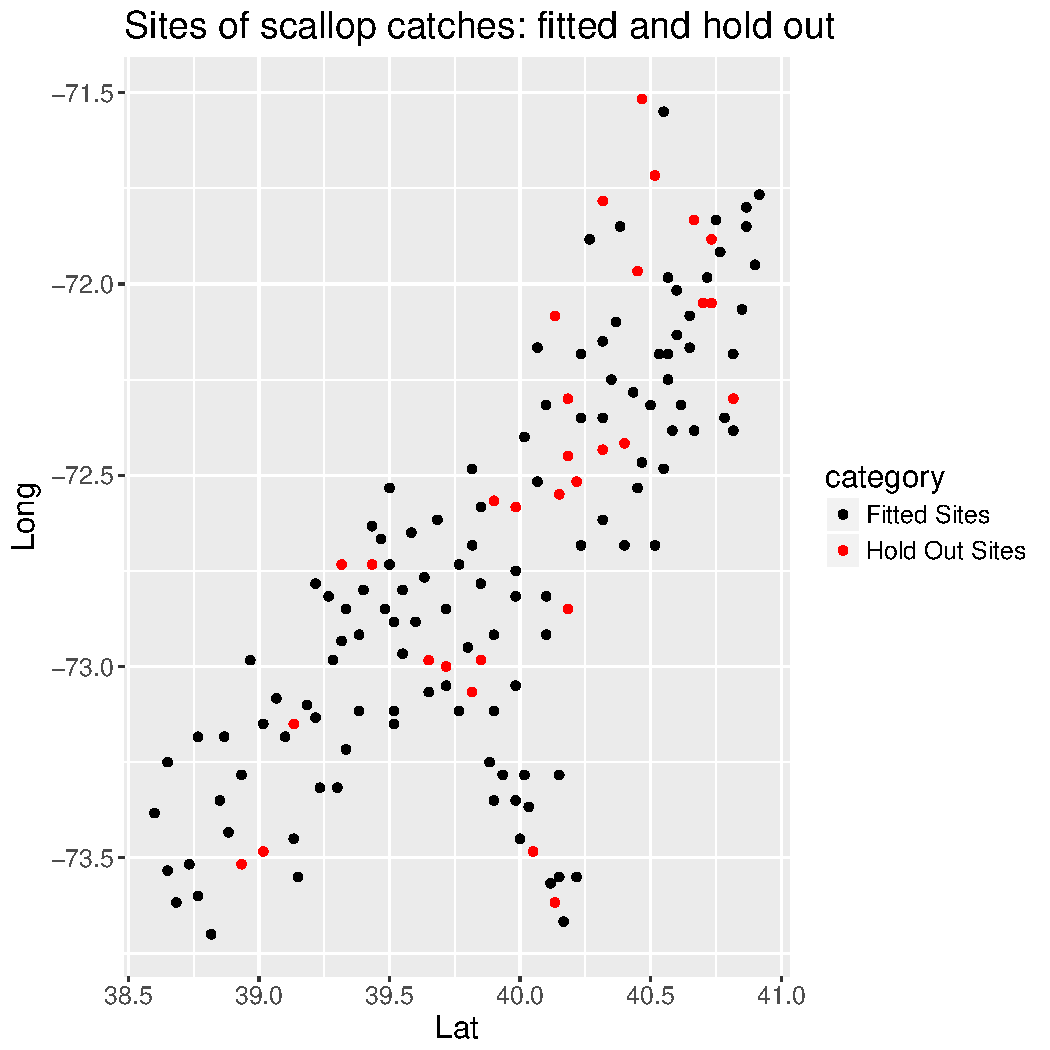
\includegraphics[scale=0.7]{figure/scallop_sites} \caption{Sites sampled in the Atlantic Ocean for 1993 scallop catch data (fitted and hold out)}\label{fig:scallop}
\end{figure}
\begin{figure}
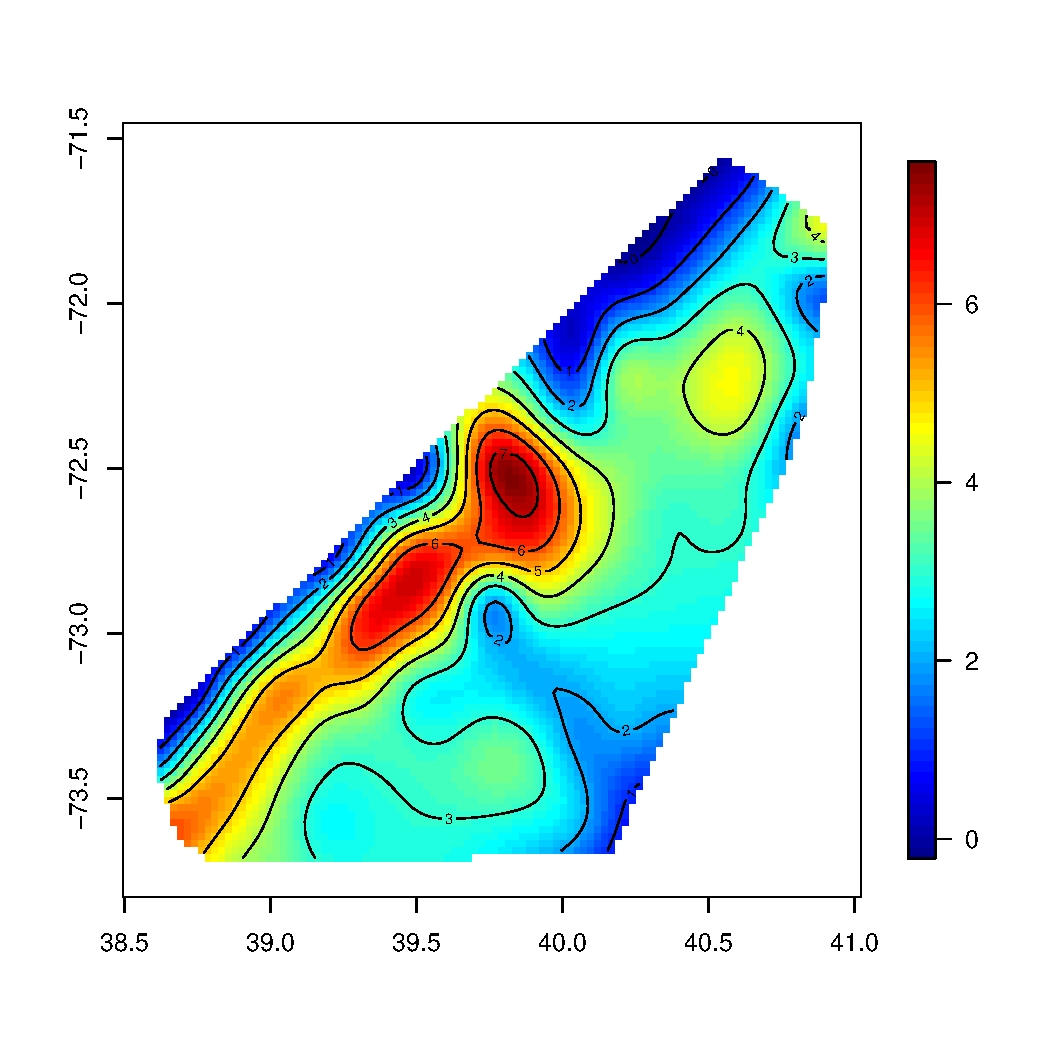
\includegraphics[scale=0.7]{figure/surface} \caption{Surface and contour plot for 1993 scallop data (fitted)}\label{fig:surf}
\end{figure}
Again, we fit the anisotropic model using methodology detailed in
section 3, and the isotropic model using spBayes. In both cases, we run
30,000 iterations, using a burn-in of 20,000 and a thinning rate of 1/20
for the remaining 10,000 samples. Therefore, we retain 500 posterior
samples of all model parameters. Figure \ref{fig:density} shows the
density plot of the remaining posterior samples under anisotropy. Table
\ref{tab:param} shows the posterior means and 95\% credible intervals
for all model parameters under isotropy and anisotropy.
\begin{figure}
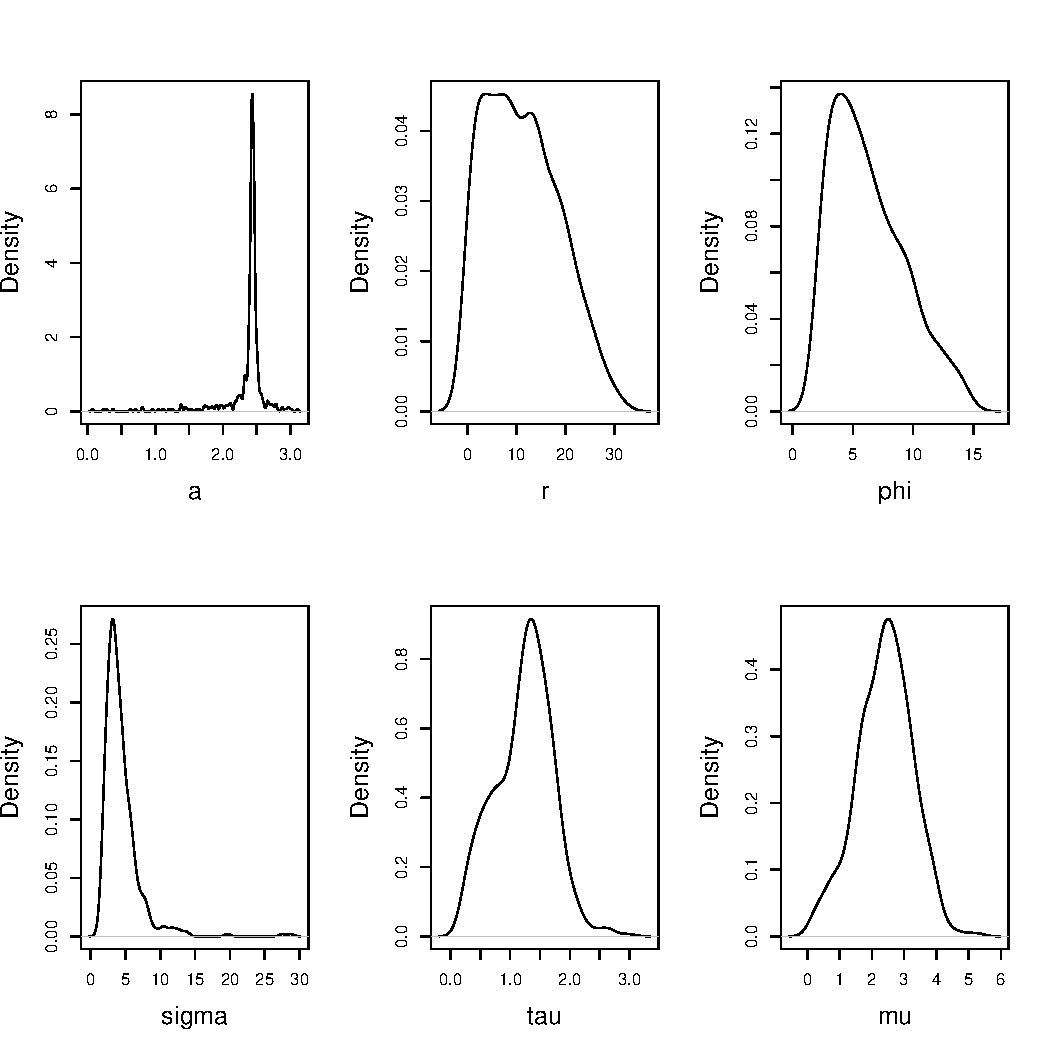
\includegraphics[scale=0.7]{figure/density} \caption{Density plots of posterior samples for all parameters under anisotropy (after burn-in and thinning)}\label{fig:density}
\end{figure}
\begin{table}[H]
\centering
\setlength{\extrarowheight}{15pt}
\hspace*{-1.2cm}
\begin{tabular}{|c|c|c|c|c|c|c|}
\hline
Parameters & $\mu$ & $\phi$ & $\sigma^2$ & $\tau^2$ & $\alpha$ & $r$ \\[10pt]
\hline
Isotropy & NA & \pbox{20cm}{4.92\\(2.49, 8.71)} & \pbox{20cm}{5.20\\(3.10, 8.94)} & \pbox{20cm}{0.49\\(0.19, 1.15)} & NA & NA \\
\hline
Anisotropy & \pbox{20cm}{2.40 \\(0.57, 3.96)} & \pbox{20cm}{6.3 \\(2.23, 13.24)} & \pbox{20cm}{4.36 \\(1.77, 10.81)} & \pbox{20cm}{1.23 \\(0.30, 2.07)} & \pbox{20cm}{2.35\\(1.31, 2.74)} & \pbox{20cm}{11.2 \\(0.49, 26.27)}\\
\hline
\end{tabular}
\caption{Posterior means and 95\% credible intervals for all model parameters under isotropy and anisotropy}
\label{tab:param}
\end{table}
To show evidence for departure from isotropy, we obtain the posterior
distribution for range in each direction. Figure \ref{fig:ranges} shows
the mean posterior range plotted as a function of angle with associated
individual 95\% credible intervals. The plot on the right shows the
range in polar coordinates which forms an ellipse.
\begin{figure}
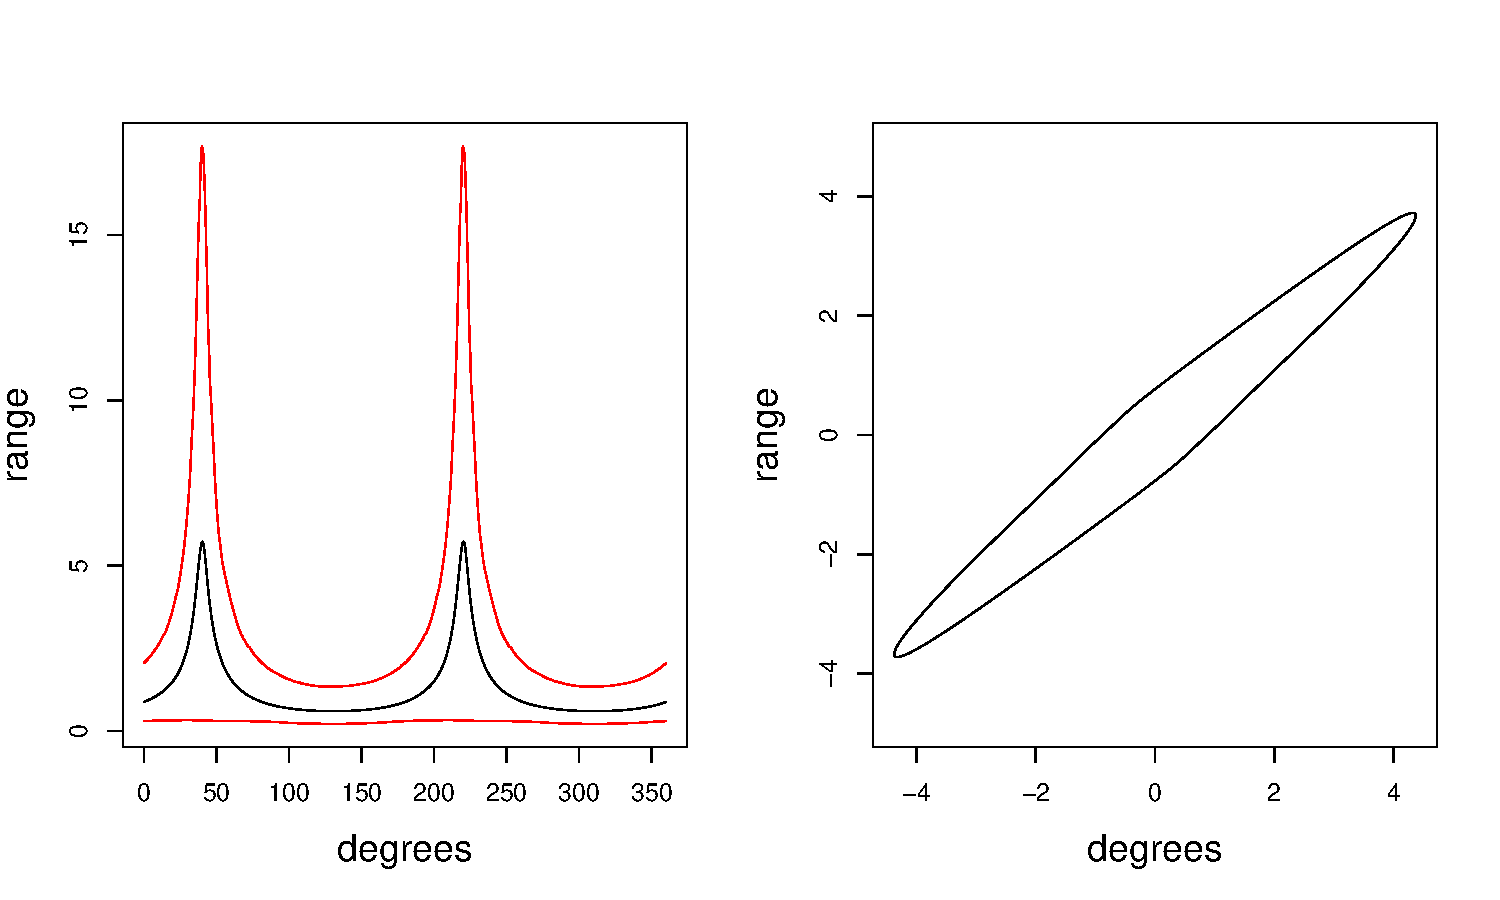
\includegraphics[scale=0.6]{figure/ranges} \caption{Mean posterior range plotted as a function of angle with associated individual 95 percent credible intervals. The plot on the right shows the range in polar coordinates which forms an ellipse.}\label{fig:ranges}
\end{figure}
We evaluate the predictive performance of the two models on the 30
hold-out sites using empirical coverage, PMSE and CRPS, as displayed in
Table \ref{tab:eval}. The anisotropic model reduces average PMSE by 12\%
and reduces average CRPS by 7\% over the 30 sites. Anisotropy also has
higher empirical coverage than isotropy.
\begin{table}[H]
\centering
\setlength{\extrarowheight}{10pt}
\begin{tabular}{|c|c|c|c|}
\hline
Model & EC & PMSE & CRPS\\[10pt]
\hline
Isotropy & 86.7\% & 1.792 & 0.781\\
\hline
Anisotropy & 96.7\% & 1.581 & 0.725 \\
\hline
\end{tabular}
\caption{Model comparison of isotropy and anisotropy for scallops data: 90\% empirical coverage, PMSE, and CRPS}
\label{tab:eval}
\end{table}
Figure \ref{fig:EC} shows the empirical coverage of isotropy and
anisotropy, where the dots represent the observed values and the grey
lines represent the 90\% credible interval of the posterior predictive
samples. We can see the credible intervals produced by isotropy fail to
capture the observed value for 4 of the 30 sites, while anisotropy fails
to capture 1 site.
\begin{figure}
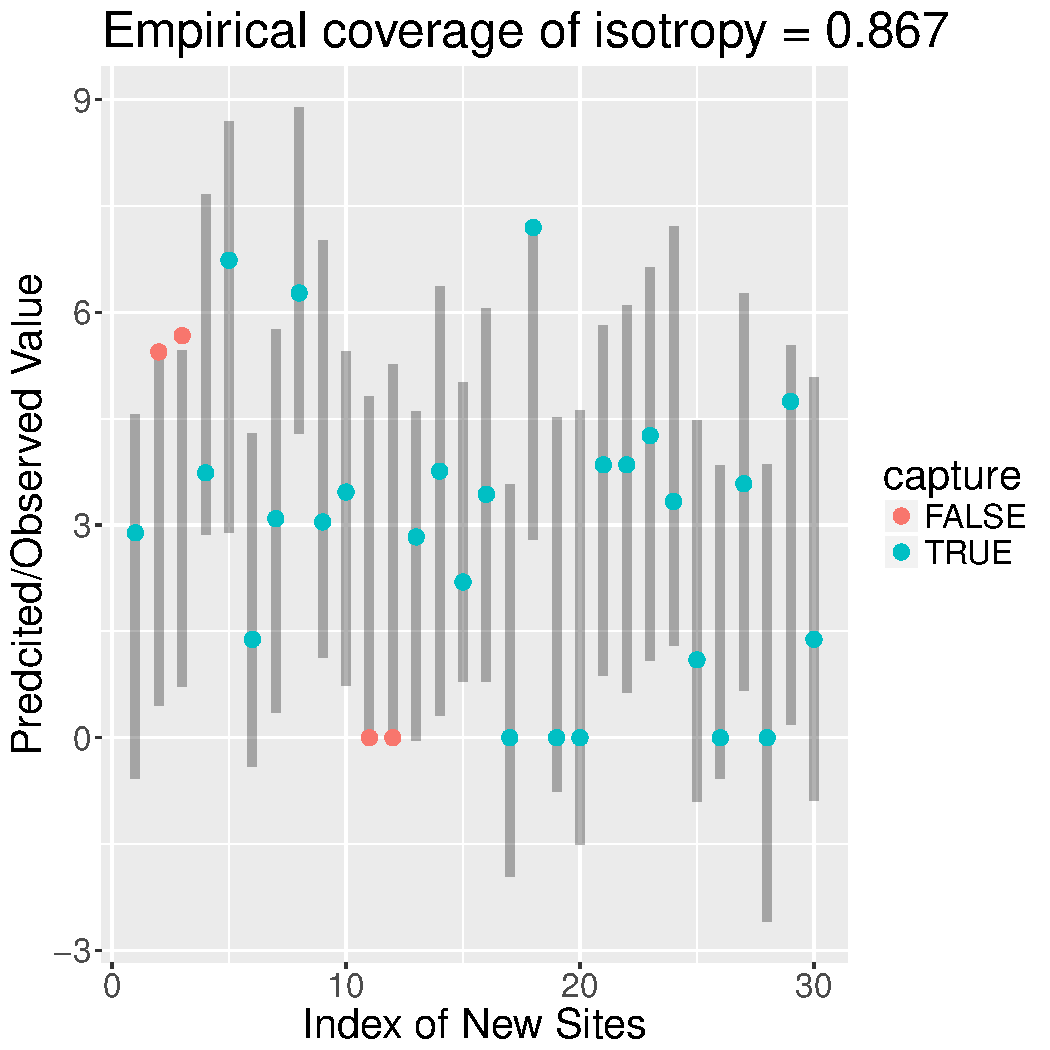
\includegraphics[scale=0.7]{figure/empCovIso} \caption{Model comparison: empirical coverage of isotropy and anisotropy}\label{fig:EC}
\end{figure}
\begin{figure}
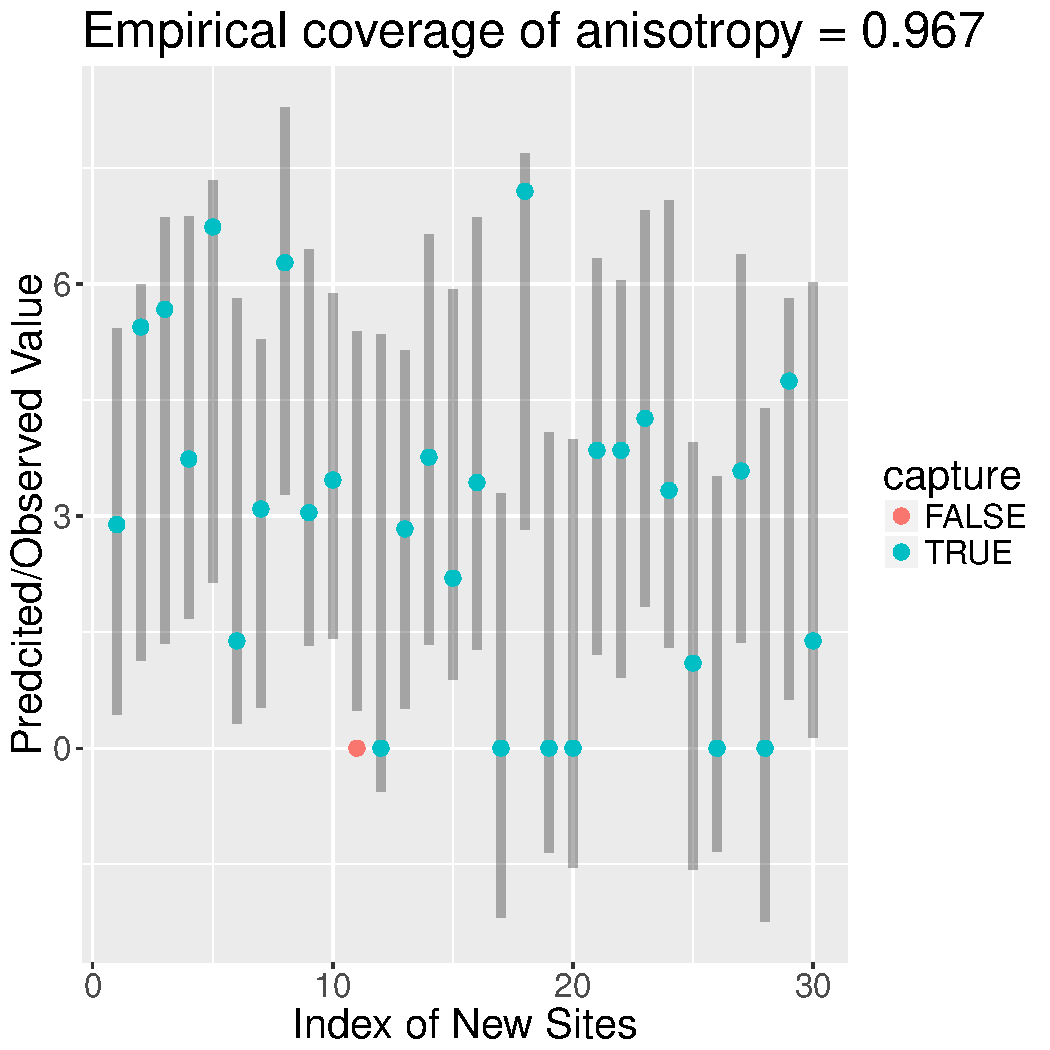
\includegraphics[scale=0.7]{figure/empCovAniso} \caption{Model comparison: empirical coverage of isotropy and anisotropy}\label{fig:EC2}
\end{figure}
Figure \ref{fig:CRPS} shows the posterior predictive distribution and
PMSE for 4 randomly selected hold out sites under isotropy and
anisotropy. The vertical line represents the observed value. Under
anisotropy, the predictive distributions are more closely concentrated
around the observed value, and the PMSE's are smaller.
\begin{figure}
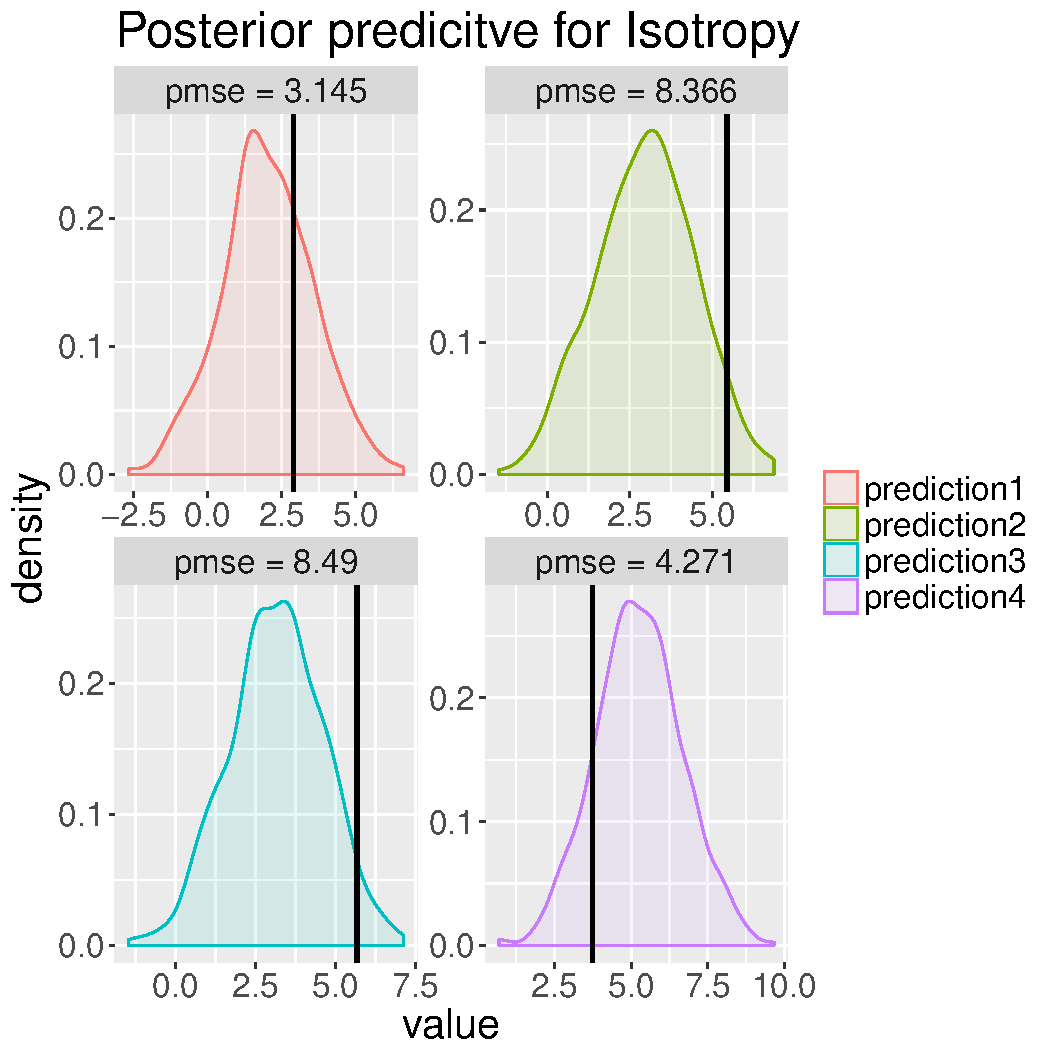
\includegraphics[scale=0.7]{figure/crps_Iso} \caption{Model comparison: posterior predictive distribution and PMSE for 4 hold out sites under isotropy and anisotropy. Vertical line represents the observed value.}\label{fig:CRPS}
\end{figure}
\begin{figure}
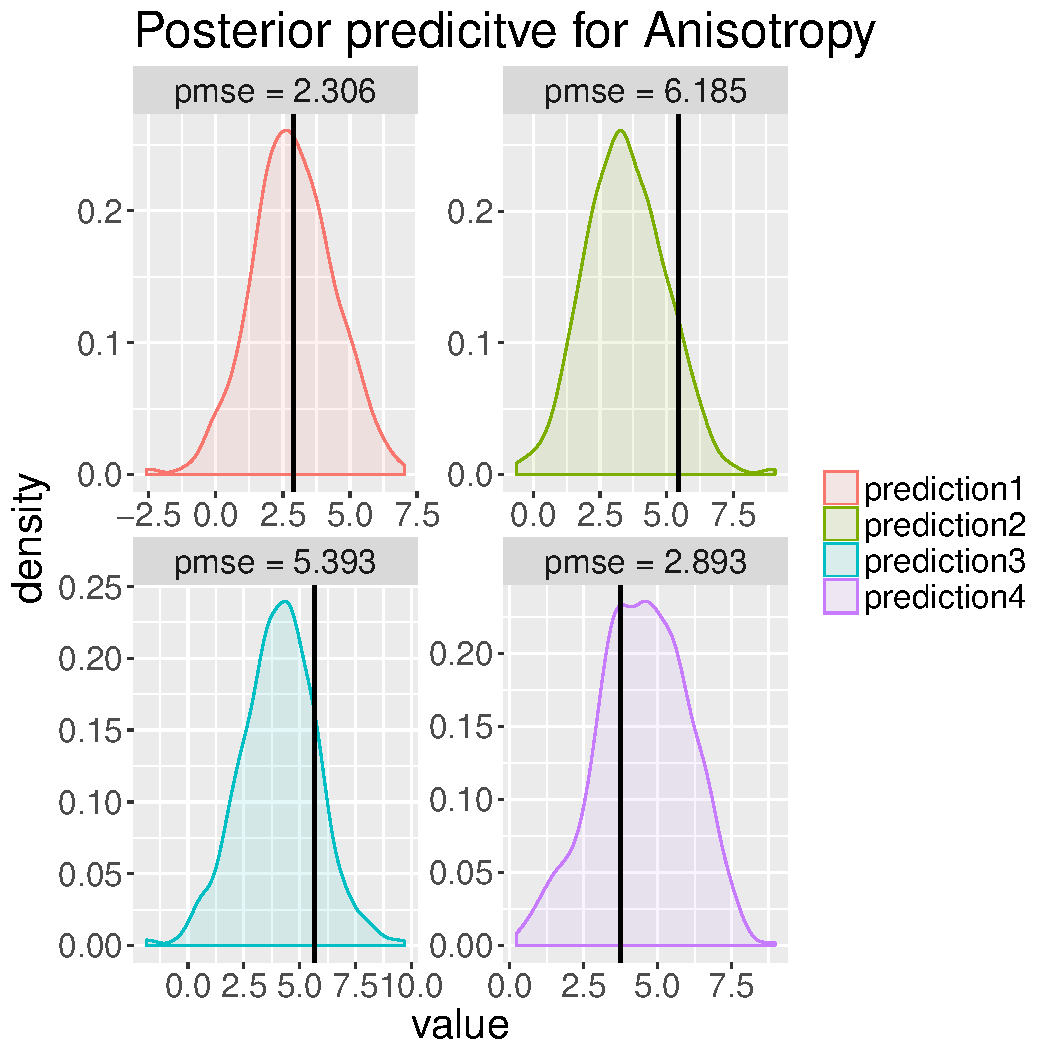
\includegraphics[scale=0.7]{figure/crps_Aniso} \caption{Model comparison: posterior predictive distribution and PMSE for 4 hold out sites under isotropy and anisotropy. Vertical line represents the observed value.}\label{fig:CRPS1}
\end{figure}
\chapter{Discussion and Future Work}\label{discussion-and-future-work}

This paper explored when and how much geometric anisotropic models for
random effects in geostatistical settings improve predictive performance
over isotropic models. We compared the predictive performance of
isotropic and anisotropic models for data generated under anisotropy,
using different values of the parameters in the data generating model,
including different sample sizes, different choices of anisotropy ratio,
and different scales and ratios of spatial variance and pure error. We
found that anisotropy yields better predictive performance when the data
significantly departs from isotropy (anisotropy ratio is much greater
than one), and that the improvement is more prominent when the
anisotropy ratio is higher and when spatial variance is higher compared
to pure error, regardless of sample size. The anisotropic model yields
much better predictive results on the real scallop catches data, which
have been suggested to exhibit anisotropic behavior. We performed full
Bayesian inference on all model parameters using a Metropolis-Hastings
algorithm for model fitting.

Future work involves extending the geometric anisotropic model
assessment to multivariate observations at locations and to space-time
settings. We will also explore different ways of constructing
stationarity by using different covariance structures. In particular we
are interested in exploring product covariance function, i.e.~the
product of one-dimensional covariance function in the x-coordinate and a
one-dimensional covariance function in the y-coordinate, which takes the
following form:
\begin{equation*}
C(d) = \begin{cases}
\tau^2 + \sigma^2 & \text{if $d=0$}\\
\sigma^2\text{exp}(-\phi_{x} d_{x})\text{exp}(-\phi_{y}d_{y}) & \text{if $d>0$}
\end{cases}
\end{equation*}
where \(d_{x}\) is the distance between x-coordinates and \(d_{y}\) is
the distance between y-coordinates.

\backmatter

\chapter*{References}\label{references}
\addcontentsline{toc}{chapter}{References}

\markboth{References}{References}

\noindent

\setlength{\parindent}{-0.20in} \setlength{\leftskip}{0.20in}
\setlength{\parskip}{8pt}

\hypertarget{refs}{}
\hypertarget{ref-ASP2016}{}
Allard, D., Senoussi, R., \& Porcu, E. (2016). Anisotropy models for
spatial data. \emph{Mathematical Geosciences}, \emph{48}(3), 305--328.

\hypertarget{ref-BCG}{}
Banerjee, S., Carlin, B. P., \& Gelfand, A. E. (2014).
\emph{Hierarchical modeling and analysis for spatial data}. Taylor;
Francis.

\hypertarget{ref-BD2005}{}
Budrikaite, L., \& Ducinskas, K. (2005). Modelling of geometric
anisotropic spatial variation. \emph{Mathematical Modeling and
Analysis}, 361--366.

\hypertarget{ref-Gelfand1999}{}
Ecker, M. D., \& Gelfand, A. E. (1999). Bayesian modeling and inference
for geometrically anisotropic spatial data. \emph{Mathematical Geology},
\emph{31}(1), 67--83.

\hypertarget{ref-Eriksson2000}{}
Eriksson, M., \& Siska, P. P. (2000). Understanding anisotropy
computations. \emph{Mathematical Geology}, \emph{32}(6), 683--700.

\hypertarget{ref-spb1}{}
Finley, A. O., Banerjee, S., \& Carlin, B. P. (2007). spBayes: An R
package for univariate and multivariate hierarchical point-referenced
spatial models. \emph{Journal of Statistical Software}, \emph{19}(4),
1--24. Retrieved from \url{http://www.jstatsoft.org/v19/i04/}

\hypertarget{ref-Hannes2013}{}
Kazianka, H. (2013). Objective bayesian analysis of geometrically
anisotropic spatial data. \emph{Journal of Agricultural, Biological, and
Environmental Statistics}, \emph{18}(4), 514--537.

\hypertarget{ref-PGM2006}{}
Porcu, E., Gregori, P., \& Mateu, J. (2006). Nonseparable stationary
anisotropic space--time covariance functions. \emph{Stochastic
Environmental Research and Risk Assessment}, \emph{21}, 113--122.

\hypertarget{ref-Z1993}{}
Zimmerman, D. L. (1993). Another look at anisotropy in geostatistcs.
\emph{Mathematical Geology}, \emph{25}(4), 453--470.


% Index?

\end{document}
